\documentclass[twoside]{book}

% Packages required by doxygen
\usepackage{fixltx2e}
\usepackage{calc}
\usepackage{doxygen}
\usepackage[export]{adjustbox} % also loads graphicx
\usepackage{graphicx}
\usepackage[utf8]{inputenc}
\usepackage{makeidx}
\usepackage{multicol}
\usepackage{multirow}
\PassOptionsToPackage{warn}{textcomp}
\usepackage{textcomp}
\usepackage[nointegrals]{wasysym}
\usepackage[table]{xcolor}

% NLS support packages
\usepackage{polski}
\usepackage[T1]{fontenc}

% Font selection
\usepackage[T1]{fontenc}
\usepackage[scaled=.90]{helvet}
\usepackage{courier}
\usepackage{amssymb}
\usepackage{sectsty}
\renewcommand{\familydefault}{\sfdefault}
\allsectionsfont{%
  \fontseries{bc}\selectfont%
  \color{darkgray}%
}
\renewcommand{\DoxyLabelFont}{%
  \fontseries{bc}\selectfont%
  \color{darkgray}%
}
\newcommand{\+}{\discretionary{\mbox{\scriptsize$\hookleftarrow$}}{}{}}

% Page & text layout
\usepackage{geometry}
\geometry{%
  a4paper,%
  top=2.5cm,%
  bottom=2.5cm,%
  left=2.5cm,%
  right=2.5cm%
}
\tolerance=750
\hfuzz=15pt
\hbadness=750
\setlength{\emergencystretch}{15pt}
\setlength{\parindent}{0cm}
\setlength{\parskip}{3ex plus 2ex minus 2ex}
\makeatletter
\renewcommand{\paragraph}{%
  \@startsection{paragraph}{4}{0ex}{-1.0ex}{1.0ex}{%
    \normalfont\normalsize\bfseries\SS@parafont%
  }%
}
\renewcommand{\subparagraph}{%
  \@startsection{subparagraph}{5}{0ex}{-1.0ex}{1.0ex}{%
    \normalfont\normalsize\bfseries\SS@subparafont%
  }%
}
\makeatother

% Headers & footers
\usepackage{fancyhdr}
\pagestyle{fancyplain}
\fancyhead[LE]{\fancyplain{}{\bfseries\thepage}}
\fancyhead[CE]{\fancyplain{}{}}
\fancyhead[RE]{\fancyplain{}{\bfseries\leftmark}}
\fancyhead[LO]{\fancyplain{}{\bfseries\rightmark}}
\fancyhead[CO]{\fancyplain{}{}}
\fancyhead[RO]{\fancyplain{}{\bfseries\thepage}}
\fancyfoot[LE]{\fancyplain{}{}}
\fancyfoot[CE]{\fancyplain{}{}}
\fancyfoot[RE]{\fancyplain{}{\bfseries\scriptsize Wygenerowano przez Doxygen }}
\fancyfoot[LO]{\fancyplain{}{\bfseries\scriptsize Wygenerowano przez Doxygen }}
\fancyfoot[CO]{\fancyplain{}{}}
\fancyfoot[RO]{\fancyplain{}{}}
\renewcommand{\footrulewidth}{0.4pt}
\renewcommand{\chaptermark}[1]{%
  \markboth{#1}{}%
}
\renewcommand{\sectionmark}[1]{%
  \markright{\thesection\ #1}%
}

% Indices & bibliography
\usepackage{natbib}
\usepackage[titles]{tocloft}
\setcounter{tocdepth}{3}
\setcounter{secnumdepth}{5}
\makeindex

% Hyperlinks (required, but should be loaded last)
\usepackage{ifpdf}
\ifpdf
  \usepackage[pdftex,pagebackref=true]{hyperref}
\else
  \usepackage[ps2pdf,pagebackref=true]{hyperref}
\fi
\hypersetup{%
  colorlinks=true,%
  linkcolor=blue,%
  citecolor=blue,%
  unicode%
}

% Custom commands
\newcommand{\clearemptydoublepage}{%
  \newpage{\pagestyle{empty}\cleardoublepage}%
}

\usepackage{caption}
\captionsetup{labelsep=space,justification=centering,font={bf},singlelinecheck=off,skip=4pt,position=top}

%===== C O N T E N T S =====

\begin{document}

% Titlepage & ToC
\hypersetup{pageanchor=false,
             bookmarksnumbered=true,
             pdfencoding=unicode
            }
\pagenumbering{alph}
\begin{titlepage}
\vspace*{7cm}
\begin{center}%
{\Large My Project }\\
\vspace*{1cm}
{\large Wygenerowano przez Doxygen 1.8.13}\\
\end{center}
\end{titlepage}
\clearemptydoublepage
\pagenumbering{roman}
\tableofcontents
\clearemptydoublepage
\pagenumbering{arabic}
\hypersetup{pageanchor=true}

%--- Begin generated contents ---
\chapter{Indeks przestrzeni nazw}
\section{Pakiety}
Oto lista pakietów wraz z krótkim opisem (o ile jest dostępny)\+:\begin{DoxyCompactList}
\item\contentsline{section}{\hyperlink{namespace_windows_forms_app2}{Windows\+Forms\+App2} }{\pageref{namespace_windows_forms_app2}}{}
\end{DoxyCompactList}

\chapter{Indeks hierarchiczny}
\section{Class Hierarchy}
This inheritance list is sorted roughly, but not completely, alphabetically\+:\begin{DoxyCompactList}
\item Form\begin{DoxyCompactList}
\item \contentsline{section}{Windows\+Forms\+App2.\+Przegladarka}{\pageref{class_windows_forms_app2_1_1_przegladarka}}{}
\item \contentsline{section}{Windows\+Forms\+App2.\+Ulubione}{\pageref{class_windows_forms_app2_1_1_ulubione}}{}
\end{DoxyCompactList}
\item \contentsline{section}{Windows\+Forms\+App2.\+Program}{\pageref{class_windows_forms_app2_1_1_program}}{}
\end{DoxyCompactList}

\chapter{Indeks klas}
\section{Class List}
Here are the classes, structs, unions and interfaces with brief descriptions\+:\begin{DoxyCompactList}
\item\contentsline{section}{\hyperlink{class_windows_forms_app2_1_1_program}{Windows\+Forms\+App2.\+Program} }{\pageref{class_windows_forms_app2_1_1_program}}{}
\item\contentsline{section}{\hyperlink{class_windows_forms_app2_1_1_przegladarka}{Windows\+Forms\+App2.\+Przegladarka} }{\pageref{class_windows_forms_app2_1_1_przegladarka}}{}
\item\contentsline{section}{\hyperlink{class_windows_forms_app2_1_1_ulubione}{Windows\+Forms\+App2.\+Ulubione} }{\pageref{class_windows_forms_app2_1_1_ulubione}}{}
\end{DoxyCompactList}

\chapter{Dokumentacja przestrzeni nazw}
\hypertarget{namespace_windows_forms_app2}{}\section{Windows\+Forms\+App2 Namespace Reference}
\label{namespace_windows_forms_app2}\index{Windows\+Forms\+App2@{Windows\+Forms\+App2}}
\subsection*{Classes}
\begin{DoxyCompactItemize}
\item 
class \hyperlink{class_windows_forms_app2_1_1_program}{Program}
\item 
class \hyperlink{class_windows_forms_app2_1_1_przegladarka}{Przegladarka}
\item 
class \hyperlink{class_windows_forms_app2_1_1_ulubione}{Ulubione}
\end{DoxyCompactItemize}

\chapter{Dokumentacja klas}
\hypertarget{class_windows_forms_app2_1_1_program}{}\section{Dokumentacja klasy Windows\+Forms\+App2.\+Program}
\label{class_windows_forms_app2_1_1_program}\index{Windows\+Forms\+App2.\+Program@{Windows\+Forms\+App2.\+Program}}
\subsection*{Statyczne metody prywatne}
\begin{DoxyCompactItemize}
\item 
static void \hyperlink{class_windows_forms_app2_1_1_program_aa742224747f9ce5e02ea3099ff23c239}{Main} ()
\begin{DoxyCompactList}\small\item\em Główny punkt wejścia dla aplikacji. \end{DoxyCompactList}\end{DoxyCompactItemize}


\subsection{Dokumentacja funkcji składowych}
\mbox{\Hypertarget{class_windows_forms_app2_1_1_program_aa742224747f9ce5e02ea3099ff23c239}\label{class_windows_forms_app2_1_1_program_aa742224747f9ce5e02ea3099ff23c239}} 
\index{Windows\+Forms\+App2\+::\+Program@{Windows\+Forms\+App2\+::\+Program}!Main@{Main}}
\index{Main@{Main}!Windows\+Forms\+App2\+::\+Program@{Windows\+Forms\+App2\+::\+Program}}
\subsubsection{\texorpdfstring{Main()}{Main()}}
{\footnotesize\ttfamily static void Windows\+Forms\+App2.\+Program.\+Main (\begin{DoxyParamCaption}{ }\end{DoxyParamCaption})\hspace{0.3cm}{\ttfamily [static]}, {\ttfamily [private]}}



Główny punkt wejścia dla aplikacji. 



Dokumentacja dla tej klasy została wygenerowana z pliku\+:\begin{DoxyCompactItemize}
\item 
Program.\+cs\end{DoxyCompactItemize}

\hypertarget{class_windows_forms_app2_1_1_przegladarka}{}\section{Windows\+Forms\+App2.\+Przegladarka Class Reference}
\label{class_windows_forms_app2_1_1_przegladarka}\index{Windows\+Forms\+App2.\+Przegladarka@{Windows\+Forms\+App2.\+Przegladarka}}
Inheritance diagram for Windows\+Forms\+App2.\+Przegladarka\+:\begin{figure}[H]
\begin{center}
\leavevmode
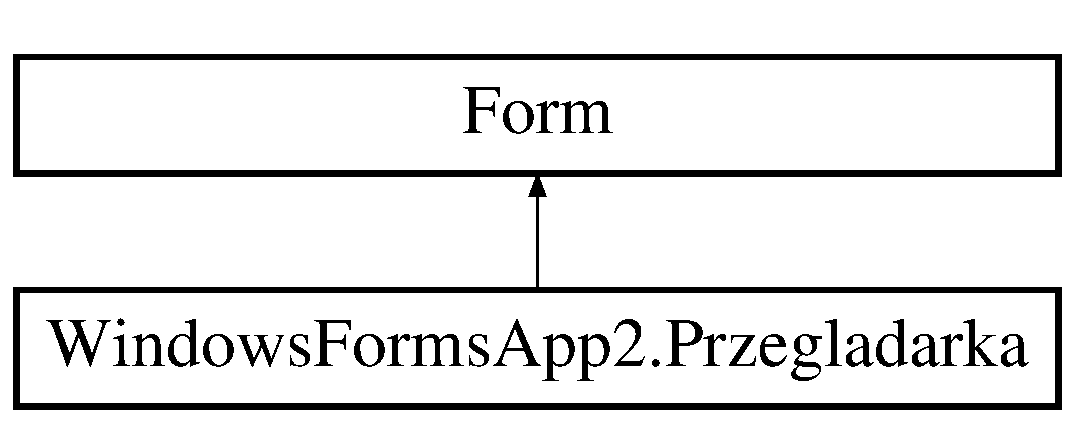
\includegraphics[height=2.000000cm]{class_windows_forms_app2_1_1_przegladarka}
\end{center}
\end{figure}
\subsection*{Static Public Member Functions}
\begin{DoxyCompactItemize}
\item 
\mbox{\Hypertarget{class_windows_forms_app2_1_1_przegladarka_a25874245b07b80396888b5c96bb67251}\label{class_windows_forms_app2_1_1_przegladarka_a25874245b07b80396888b5c96bb67251}} 
static Image \hyperlink{class_windows_forms_app2_1_1_przegladarka_a25874245b07b80396888b5c96bb67251}{favicon} (String u, string file)
\begin{DoxyCompactList}\small\item\em favicon \end{DoxyCompactList}\end{DoxyCompactItemize}
\subsection*{Static Public Attributes}
\begin{DoxyCompactItemize}
\item 
\mbox{\Hypertarget{class_windows_forms_app2_1_1_przegladarka_ab28068e2ce99fd06715ca76c9d1ba6ca}\label{class_windows_forms_app2_1_1_przegladarka_ab28068e2ce99fd06715ca76c9d1ba6ca}} 
static String {\bfseries fav\+Xml} = \char`\"{}favorits.\+xml\char`\"{}
\end{DoxyCompactItemize}
\subsection*{Protected Member Functions}
\begin{DoxyCompactItemize}
\item 
override void \hyperlink{class_windows_forms_app2_1_1_przegladarka_a1952e96668e9dae2dd62a80771162925}{Dispose} (bool disposing)
\begin{DoxyCompactList}\small\item\em Wyczyść wszystkie używane zasoby. \end{DoxyCompactList}\end{DoxyCompactItemize}
\subsection*{Private Member Functions}
\begin{DoxyCompactItemize}
\item 
\mbox{\Hypertarget{class_windows_forms_app2_1_1_przegladarka_a7d52cb2619b2a3c247a6f420ee7a6ef4}\label{class_windows_forms_app2_1_1_przegladarka_a7d52cb2619b2a3c247a6f420ee7a6ef4}} 
void {\bfseries Form1\+\_\+\+Load} (object sender, Event\+Args e)
\item 
void \hyperlink{class_windows_forms_app2_1_1_przegladarka_ae81e3a8848fdaaecd2f51a2f17e60540}{add\+Favorit} (String url, string name)
\item 
\mbox{\Hypertarget{class_windows_forms_app2_1_1_przegladarka_a317944e036dffa9dbae17e072ffce939}\label{class_windows_forms_app2_1_1_przegladarka_a317944e036dffa9dbae17e072ffce939}} 
void \hyperlink{class_windows_forms_app2_1_1_przegladarka_a317944e036dffa9dbae17e072ffce939}{add\+Link} (String url, string name)
\begin{DoxyCompactList}\small\item\em Pasek szybkiego dostepu. \end{DoxyCompactList}\item 
\mbox{\Hypertarget{class_windows_forms_app2_1_1_przegladarka_a09bd06ccc833afe04008333d58e873b1}\label{class_windows_forms_app2_1_1_przegladarka_a09bd06ccc833afe04008333d58e873b1}} 
void \hyperlink{class_windows_forms_app2_1_1_przegladarka_a09bd06ccc833afe04008333d58e873b1}{items\+\_\+\+Click} (object sender, Event\+Args e)
\begin{DoxyCompactList}\small\item\em click link button \end{DoxyCompactList}\item 
\mbox{\Hypertarget{class_windows_forms_app2_1_1_przegladarka_a263c2982999a825c5df27a3d0394f8a6}\label{class_windows_forms_app2_1_1_przegladarka_a263c2982999a825c5df27a3d0394f8a6}} 
void \hyperlink{class_windows_forms_app2_1_1_przegladarka_a263c2982999a825c5df27a3d0394f8a6}{b\+\_\+\+Mouse\+Up} (object sender, Mouse\+Event\+Args e)
\begin{DoxyCompactList}\small\item\em show context menu on button \end{DoxyCompactList}\item 
\mbox{\Hypertarget{class_windows_forms_app2_1_1_przegladarka_a7ebc793c65547468c33de98bca06db2f}\label{class_windows_forms_app2_1_1_przegladarka_a7ebc793c65547468c33de98bca06db2f}} 
int {\bfseries favicon\+Index} (string url)
\item 
\mbox{\Hypertarget{class_windows_forms_app2_1_1_przegladarka_a6d41c318a647f8a1054fdbe57c3c132a}\label{class_windows_forms_app2_1_1_przegladarka_a6d41c318a647f8a1054fdbe57c3c132a}} 
Image {\bfseries get\+Favicon} (string key)
\item 
\mbox{\Hypertarget{class_windows_forms_app2_1_1_przegladarka_a4d940c14c495053bb984ff254991afbc}\label{class_windows_forms_app2_1_1_przegladarka_a4d940c14c495053bb984ff254991afbc}} 
Web\+Browser \hyperlink{class_windows_forms_app2_1_1_przegladarka_a4d940c14c495053bb984ff254991afbc}{get\+Current\+Browser} ()
\begin{DoxyCompactList}\small\item\em A\+D\+D\+R\+E\+SS B\+AR. \end{DoxyCompactList}\item 
\mbox{\Hypertarget{class_windows_forms_app2_1_1_przegladarka_a2c16d9618e633748a8a7eb8c3daa6dc7}\label{class_windows_forms_app2_1_1_przegladarka_a2c16d9618e633748a8a7eb8c3daa6dc7}} 
void {\bfseries adr\+Bar\+Text\+Box\+\_\+\+Key\+Down} (object sender, Key\+Event\+Args e)
\item 
\mbox{\Hypertarget{class_windows_forms_app2_1_1_przegladarka_ab0b9d9fb2c8ac43d3db70ed17e913813}\label{class_windows_forms_app2_1_1_przegladarka_ab0b9d9fb2c8ac43d3db70ed17e913813}} 
void {\bfseries Web\+\_\+\+Document\+Completed} (object sender, Web\+Browser\+Document\+Completed\+Event\+Args e)
\item 
\mbox{\Hypertarget{class_windows_forms_app2_1_1_przegladarka_a0426aa03eb6aa34e371a649c317a6995}\label{class_windows_forms_app2_1_1_przegladarka_a0426aa03eb6aa34e371a649c317a6995}} 
void \hyperlink{class_windows_forms_app2_1_1_przegladarka_a0426aa03eb6aa34e371a649c317a6995}{przejdz\+Tool\+Strip\+Menu\+Item\+\_\+\+Click} (object sender, Event\+Args e)
\begin{DoxyCompactList}\small\item\em L\+OG. \end{DoxyCompactList}\item 
\mbox{\Hypertarget{class_windows_forms_app2_1_1_przegladarka_add440881c3f047aa654c6e992f84dac8}\label{class_windows_forms_app2_1_1_przegladarka_add440881c3f047aa654c6e992f84dac8}} 
void {\bfseries wstecz\+Tool\+Strip\+Menu\+Item\+\_\+\+Click} (object sender, Event\+Args e)
\item 
\mbox{\Hypertarget{class_windows_forms_app2_1_1_przegladarka_a6e7bcbe6a5b31132e29787c80b663d02}\label{class_windows_forms_app2_1_1_przegladarka_a6e7bcbe6a5b31132e29787c80b663d02}} 
void {\bfseries tool\+Strip\+Menu\+Item1\+\_\+\+Click} (object sender, Event\+Args e)
\item 
\mbox{\Hypertarget{class_windows_forms_app2_1_1_przegladarka_a1a65fd7d680f3af4d036af3992129a81}\label{class_windows_forms_app2_1_1_przegladarka_a1a65fd7d680f3af4d036af3992129a81}} 
void \hyperlink{class_windows_forms_app2_1_1_przegladarka_a1a65fd7d680f3af4d036af3992129a81}{dodaj\+Karte\+Tool\+Strip\+Menu\+Item\+\_\+\+Click} (object sender, Event\+Args e)
\begin{DoxyCompactList}\small\item\em A\+DD C\+A\+RD. \end{DoxyCompactList}\item 
\mbox{\Hypertarget{class_windows_forms_app2_1_1_przegladarka_ac405fedd591d91fba5dadc8d0b3b2419}\label{class_windows_forms_app2_1_1_przegladarka_ac405fedd591d91fba5dadc8d0b3b2419}} 
void \hyperlink{class_windows_forms_app2_1_1_przegladarka_ac405fedd591d91fba5dadc8d0b3b2419}{usuń\+Karte\+Tool\+Strip\+Menu\+Item\+\_\+\+Click} (object sender, Event\+Args e)
\begin{DoxyCompactList}\small\item\em D\+E\+L\+E\+TE C\+A\+RD. \end{DoxyCompactList}\item 
\mbox{\Hypertarget{class_windows_forms_app2_1_1_przegladarka_a1b8caaa571e0f20423e36048bebe658d}\label{class_windows_forms_app2_1_1_przegladarka_a1b8caaa571e0f20423e36048bebe658d}} 
void {\bfseries tab\+Control1\+\_\+\+Selected\+Index\+Changed} (object sender, Event\+Args e)
\item 
\mbox{\Hypertarget{class_windows_forms_app2_1_1_przegladarka_a7c9a987ad2c6d99e4b8744247939b447}\label{class_windows_forms_app2_1_1_przegladarka_a7c9a987ad2c6d99e4b8744247939b447}} 
void {\bfseries tool\+Strip\+Combo\+Box1\+\_\+\+Click} (object sender, Event\+Args e)
\item 
\mbox{\Hypertarget{class_windows_forms_app2_1_1_przegladarka_a44c5511659d6a003813e4efc5308a69c}\label{class_windows_forms_app2_1_1_przegladarka_a44c5511659d6a003813e4efc5308a69c}} 
void \hyperlink{class_windows_forms_app2_1_1_przegladarka_a44c5511659d6a003813e4efc5308a69c}{dodaj\+Tool\+Strip\+Menu\+Item\+\_\+\+Click} (object sender, Event\+Args e)
\begin{DoxyCompactList}\small\item\em U\+L\+U\+B\+I\+O\+NE. \end{DoxyCompactList}\item 
void \hyperlink{class_windows_forms_app2_1_1_przegladarka_a16d94dcbfce3b5319ae8b36f0d9fe26b}{Initialize\+Component} ()
\begin{DoxyCompactList}\small\item\em Metoda wymagana do obsługi projektanta — nie należy modyfikować jej zawartości w edytorze kodu. \end{DoxyCompactList}\end{DoxyCompactItemize}
\subsection*{Private Attributes}
\begin{DoxyCompactItemize}
\item 
\mbox{\Hypertarget{class_windows_forms_app2_1_1_przegladarka_a4e6b33e38a6f98f8b3202ee9d5388060}\label{class_windows_forms_app2_1_1_przegladarka_a4e6b33e38a6f98f8b3202ee9d5388060}} 
List$<$ String $>$ {\bfseries urls} = new List$<$String$>$()
\item 
\mbox{\Hypertarget{class_windows_forms_app2_1_1_przegladarka_a6d8a0bbfaf93459ed58e74f1574613a8}\label{class_windows_forms_app2_1_1_przegladarka_a6d8a0bbfaf93459ed58e74f1574613a8}} 
Xml\+Document {\bfseries settings} = new Xml\+Document()
\item 
\mbox{\Hypertarget{class_windows_forms_app2_1_1_przegladarka_a27d7a3016562096e7921af6ce7aada19}\label{class_windows_forms_app2_1_1_przegladarka_a27d7a3016562096e7921af6ce7aada19}} 
String {\bfseries home\+Page}
\item 
\mbox{\Hypertarget{class_windows_forms_app2_1_1_przegladarka_ad655150adfd804d9faebd51a6da14e9d}\label{class_windows_forms_app2_1_1_przegladarka_ad655150adfd804d9faebd51a6da14e9d}} 
Culture\+Info {\bfseries current\+Culture}
\item 
\mbox{\Hypertarget{class_windows_forms_app2_1_1_przegladarka_a667aaf337588647c9aa1b83e4276342c}\label{class_windows_forms_app2_1_1_przegladarka_a667aaf337588647c9aa1b83e4276342c}} 
Web\+Browser {\bfseries web} = new Web\+Browser()
\item 
\mbox{\Hypertarget{class_windows_forms_app2_1_1_przegladarka_a8966d3dd2130d3703ab0996b207fd962}\label{class_windows_forms_app2_1_1_przegladarka_a8966d3dd2130d3703ab0996b207fd962}} 
int {\bfseries i} = 0
\item 
\mbox{\Hypertarget{class_windows_forms_app2_1_1_przegladarka_ab7e4a0fbc445af3c0efd986ce799814e}\label{class_windows_forms_app2_1_1_przegladarka_ab7e4a0fbc445af3c0efd986ce799814e}} 
string \hyperlink{class_windows_forms_app2_1_1_przegladarka_ab7e4a0fbc445af3c0efd986ce799814e}{adress}
\begin{DoxyCompactList}\small\item\em L\+I\+N\+KS B\+AR. \end{DoxyCompactList}\item 
\mbox{\Hypertarget{class_windows_forms_app2_1_1_przegladarka_ab013f26b227dcbe75ffe19787a524122}\label{class_windows_forms_app2_1_1_przegladarka_ab013f26b227dcbe75ffe19787a524122}} 
string {\bfseries name}
\item 
System.\+Component\+Model.\+I\+Container \hyperlink{class_windows_forms_app2_1_1_przegladarka_a37fd573e6d383f202dbea9da1940a947}{components} = null
\begin{DoxyCompactList}\small\item\em Wymagana zmienna projektanta. \end{DoxyCompactList}\item 
\mbox{\Hypertarget{class_windows_forms_app2_1_1_przegladarka_a2a73e12868cd6458c615db8cdf4bb065}\label{class_windows_forms_app2_1_1_przegladarka_a2a73e12868cd6458c615db8cdf4bb065}} 
System.\+Windows.\+Forms.\+Menu\+Strip {\bfseries menu\+Strip1}
\item 
\mbox{\Hypertarget{class_windows_forms_app2_1_1_przegladarka_adeee418fd4c8b86a5fc5139164bf98ba}\label{class_windows_forms_app2_1_1_przegladarka_adeee418fd4c8b86a5fc5139164bf98ba}} 
System.\+Windows.\+Forms.\+Tool\+Strip\+Menu\+Item {\bfseries adres\+Tool\+Strip\+Menu\+Item}
\item 
\mbox{\Hypertarget{class_windows_forms_app2_1_1_przegladarka_af586dc21d800941eb565080947eafd55}\label{class_windows_forms_app2_1_1_przegladarka_af586dc21d800941eb565080947eafd55}} 
System.\+Windows.\+Forms.\+Tool\+Strip\+Combo\+Box {\bfseries tool\+Strip\+Combo\+Box1}
\item 
\mbox{\Hypertarget{class_windows_forms_app2_1_1_przegladarka_afeb83789a4b241702af05d7fae1f6f99}\label{class_windows_forms_app2_1_1_przegladarka_afeb83789a4b241702af05d7fae1f6f99}} 
System.\+Windows.\+Forms.\+Tool\+Strip\+Menu\+Item {\bfseries przejdz\+Tool\+Strip\+Menu\+Item}
\item 
\mbox{\Hypertarget{class_windows_forms_app2_1_1_przegladarka_a559c195b9b163e11b978d6dc9140118e}\label{class_windows_forms_app2_1_1_przegladarka_a559c195b9b163e11b978d6dc9140118e}} 
System.\+Windows.\+Forms.\+Tool\+Strip\+Menu\+Item {\bfseries wstecz\+Tool\+Strip\+Menu\+Item}
\item 
\mbox{\Hypertarget{class_windows_forms_app2_1_1_przegladarka_a06bd930ae9502e3130812c6e949d034e}\label{class_windows_forms_app2_1_1_przegladarka_a06bd930ae9502e3130812c6e949d034e}} 
System.\+Windows.\+Forms.\+Tool\+Strip\+Menu\+Item {\bfseries tool\+Strip\+Menu\+Item1}
\item 
\mbox{\Hypertarget{class_windows_forms_app2_1_1_przegladarka_aa847ef973d76583fad06069687cbde08}\label{class_windows_forms_app2_1_1_przegladarka_aa847ef973d76583fad06069687cbde08}} 
System.\+Windows.\+Forms.\+Tool\+Strip\+Menu\+Item {\bfseries dodaj\+Karte\+Tool\+Strip\+Menu\+Item}
\item 
\mbox{\Hypertarget{class_windows_forms_app2_1_1_przegladarka_a57bf4cc0dbb4b2cb91cd72013b7e69ca}\label{class_windows_forms_app2_1_1_przegladarka_a57bf4cc0dbb4b2cb91cd72013b7e69ca}} 
System.\+Windows.\+Forms.\+Tool\+Strip\+Menu\+Item {\bfseries usuń\+Karte\+Tool\+Strip\+Menu\+Item}
\item 
\mbox{\Hypertarget{class_windows_forms_app2_1_1_przegladarka_ad7aa576ee790c104bf466d5609e5b4be}\label{class_windows_forms_app2_1_1_przegladarka_ad7aa576ee790c104bf466d5609e5b4be}} 
System.\+Windows.\+Forms.\+Tab\+Control {\bfseries tab\+Control1}
\item 
\mbox{\Hypertarget{class_windows_forms_app2_1_1_przegladarka_ad3a5df3b81ffdc3098dcc527b4e4bcc2}\label{class_windows_forms_app2_1_1_przegladarka_ad3a5df3b81ffdc3098dcc527b4e4bcc2}} 
System.\+Windows.\+Forms.\+Tab\+Control {\bfseries tab\+Control2}
\item 
\mbox{\Hypertarget{class_windows_forms_app2_1_1_przegladarka_a9f4f2dd866a9feaaf7dc9485c19cfe75}\label{class_windows_forms_app2_1_1_przegladarka_a9f4f2dd866a9feaaf7dc9485c19cfe75}} 
System.\+Windows.\+Forms.\+Panel {\bfseries favorites\+Panel}
\item 
\mbox{\Hypertarget{class_windows_forms_app2_1_1_przegladarka_a5d68cce2771648ea7792cd0c9c9adea0}\label{class_windows_forms_app2_1_1_przegladarka_a5d68cce2771648ea7792cd0c9c9adea0}} 
System.\+Windows.\+Forms.\+Tool\+Strip\+Menu\+Item {\bfseries dodaj\+Tool\+Strip\+Menu\+Item}
\item 
\mbox{\Hypertarget{class_windows_forms_app2_1_1_przegladarka_a06f7e91f44509f310e084393ad82b2e3}\label{class_windows_forms_app2_1_1_przegladarka_a06f7e91f44509f310e084393ad82b2e3}} 
System.\+Windows.\+Forms.\+Context\+Menu\+Strip {\bfseries fav\+Context\+Menu}
\item 
\mbox{\Hypertarget{class_windows_forms_app2_1_1_przegladarka_ae3fff43a3e2a7dda4a7841f079a60fd4}\label{class_windows_forms_app2_1_1_przegladarka_ae3fff43a3e2a7dda4a7841f079a60fd4}} 
System.\+Windows.\+Forms.\+Tab\+Page {\bfseries tab\+Page2}
\item 
\mbox{\Hypertarget{class_windows_forms_app2_1_1_przegladarka_a8f1855a5829eecb2c52be4d086b2d546}\label{class_windows_forms_app2_1_1_przegladarka_a8f1855a5829eecb2c52be4d086b2d546}} 
System.\+Windows.\+Forms.\+Tree\+View {\bfseries tree\+View1}
\item 
\mbox{\Hypertarget{class_windows_forms_app2_1_1_przegladarka_ab7162215196c1e2ea01bb2e1e7678484}\label{class_windows_forms_app2_1_1_przegladarka_ab7162215196c1e2ea01bb2e1e7678484}} 
System.\+Windows.\+Forms.\+Tool\+Strip {\bfseries link\+Bar}
\item 
\mbox{\Hypertarget{class_windows_forms_app2_1_1_przegladarka_a58d094443f963458b2a8e5e3e5162d5f}\label{class_windows_forms_app2_1_1_przegladarka_a58d094443f963458b2a8e5e3e5162d5f}} 
System.\+Windows.\+Forms.\+Context\+Menu\+Strip {\bfseries link\+Context\+Menu}
\item 
\mbox{\Hypertarget{class_windows_forms_app2_1_1_przegladarka_a993a0596a743eccff0a5a6e487821bcd}\label{class_windows_forms_app2_1_1_przegladarka_a993a0596a743eccff0a5a6e487821bcd}} 
System.\+Windows.\+Forms.\+Image\+List {\bfseries img\+List}
\end{DoxyCompactItemize}
\subsection*{Static Private Attributes}
\begin{DoxyCompactItemize}
\item 
\mbox{\Hypertarget{class_windows_forms_app2_1_1_przegladarka_abef2d22eb265cae84b4100b314e8947f}\label{class_windows_forms_app2_1_1_przegladarka_abef2d22eb265cae84b4100b314e8947f}} 
static String {\bfseries links\+Xml} = \char`\"{}links.\+xml\char`\"{}
\end{DoxyCompactItemize}


\subsection{Member Function Documentation}
\mbox{\Hypertarget{class_windows_forms_app2_1_1_przegladarka_ae81e3a8848fdaaecd2f51a2f17e60540}\label{class_windows_forms_app2_1_1_przegladarka_ae81e3a8848fdaaecd2f51a2f17e60540}} 
\index{Windows\+Forms\+App2\+::\+Przegladarka@{Windows\+Forms\+App2\+::\+Przegladarka}!add\+Favorit@{add\+Favorit}}
\index{add\+Favorit@{add\+Favorit}!Windows\+Forms\+App2\+::\+Przegladarka@{Windows\+Forms\+App2\+::\+Przegladarka}}
\subsubsection{\texorpdfstring{add\+Favorit()}{addFavorit()}}
{\footnotesize\ttfamily void Windows\+Forms\+App2.\+Przegladarka.\+add\+Favorit (\begin{DoxyParamCaption}\item[{String}]{url,  }\item[{string}]{name }\end{DoxyParamCaption})\hspace{0.3cm}{\ttfamily [private]}}

\textbackslash{}brief Lista ulubione \mbox{\Hypertarget{class_windows_forms_app2_1_1_przegladarka_a1952e96668e9dae2dd62a80771162925}\label{class_windows_forms_app2_1_1_przegladarka_a1952e96668e9dae2dd62a80771162925}} 
\index{Windows\+Forms\+App2\+::\+Przegladarka@{Windows\+Forms\+App2\+::\+Przegladarka}!Dispose@{Dispose}}
\index{Dispose@{Dispose}!Windows\+Forms\+App2\+::\+Przegladarka@{Windows\+Forms\+App2\+::\+Przegladarka}}
\subsubsection{\texorpdfstring{Dispose()}{Dispose()}}
{\footnotesize\ttfamily override void Windows\+Forms\+App2.\+Przegladarka.\+Dispose (\begin{DoxyParamCaption}\item[{bool}]{disposing }\end{DoxyParamCaption})\hspace{0.3cm}{\ttfamily [protected]}}



Wyczyść wszystkie używane zasoby. 


\begin{DoxyParams}{Parameters}
{\em disposing} & prawda, jeżeli zarządzane zasoby powinny zostać zlikwidowane; Fałsz w przeciwnym wypadku.\\
\hline
\end{DoxyParams}
\mbox{\Hypertarget{class_windows_forms_app2_1_1_przegladarka_a16d94dcbfce3b5319ae8b36f0d9fe26b}\label{class_windows_forms_app2_1_1_przegladarka_a16d94dcbfce3b5319ae8b36f0d9fe26b}} 
\index{Windows\+Forms\+App2\+::\+Przegladarka@{Windows\+Forms\+App2\+::\+Przegladarka}!Initialize\+Component@{Initialize\+Component}}
\index{Initialize\+Component@{Initialize\+Component}!Windows\+Forms\+App2\+::\+Przegladarka@{Windows\+Forms\+App2\+::\+Przegladarka}}
\subsubsection{\texorpdfstring{Initialize\+Component()}{InitializeComponent()}}
{\footnotesize\ttfamily void Windows\+Forms\+App2.\+Przegladarka.\+Initialize\+Component (\begin{DoxyParamCaption}{ }\end{DoxyParamCaption})\hspace{0.3cm}{\ttfamily [private]}}



Metoda wymagana do obsługi projektanta — nie należy modyfikować jej zawartości w edytorze kodu. 



\subsection{Member Data Documentation}
\mbox{\Hypertarget{class_windows_forms_app2_1_1_przegladarka_a37fd573e6d383f202dbea9da1940a947}\label{class_windows_forms_app2_1_1_przegladarka_a37fd573e6d383f202dbea9da1940a947}} 
\index{Windows\+Forms\+App2\+::\+Przegladarka@{Windows\+Forms\+App2\+::\+Przegladarka}!components@{components}}
\index{components@{components}!Windows\+Forms\+App2\+::\+Przegladarka@{Windows\+Forms\+App2\+::\+Przegladarka}}
\subsubsection{\texorpdfstring{components}{components}}
{\footnotesize\ttfamily System.\+Component\+Model.\+I\+Container Windows\+Forms\+App2.\+Przegladarka.\+components = null\hspace{0.3cm}{\ttfamily [private]}}



Wymagana zmienna projektanta. 



The documentation for this class was generated from the following files\+:\begin{DoxyCompactItemize}
\item 
Form1.\+cs\item 
Form1.\+Designer.\+cs\end{DoxyCompactItemize}

\hypertarget{class_windows_forms_app2_1_1_ulubione}{}\section{Windows\+Forms\+App2.\+Ulubione Class Reference}
\label{class_windows_forms_app2_1_1_ulubione}\index{Windows\+Forms\+App2.\+Ulubione@{Windows\+Forms\+App2.\+Ulubione}}
Inheritance diagram for Windows\+Forms\+App2.\+Ulubione\+:\begin{figure}[H]
\begin{center}
\leavevmode
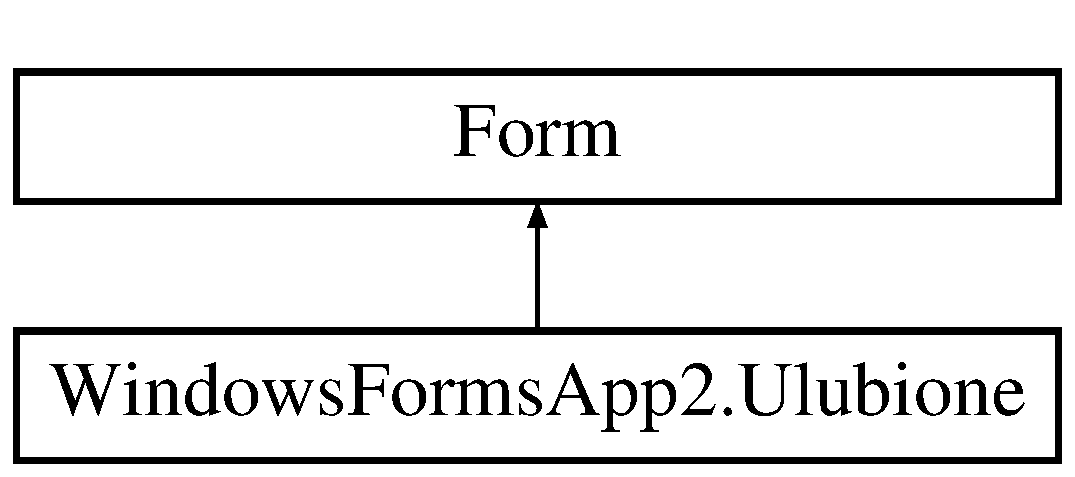
\includegraphics[height=2.000000cm]{class_windows_forms_app2_1_1_ulubione}
\end{center}
\end{figure}
\subsection*{Public Member Functions}
\begin{DoxyCompactItemize}
\item 
\mbox{\Hypertarget{class_windows_forms_app2_1_1_ulubione_a96147b868bb18d06532d4ccda7e61983}\label{class_windows_forms_app2_1_1_ulubione_a96147b868bb18d06532d4ccda7e61983}} 
{\bfseries Ulubione} (String url)
\end{DoxyCompactItemize}
\subsection*{Public Attributes}
\begin{DoxyCompactItemize}
\item 
\mbox{\Hypertarget{class_windows_forms_app2_1_1_ulubione_a164751d342358e85dc72a22ae90ecc17}\label{class_windows_forms_app2_1_1_ulubione_a164751d342358e85dc72a22ae90ecc17}} 
String {\bfseries fav\+Name}
\end{DoxyCompactItemize}
\subsection*{Protected Member Functions}
\begin{DoxyCompactItemize}
\item 
override void \hyperlink{class_windows_forms_app2_1_1_ulubione_a114b27b249c5a38d47009008fbba7ecb}{Dispose} (bool disposing)
\begin{DoxyCompactList}\small\item\em Clean up any resources being used. \end{DoxyCompactList}\end{DoxyCompactItemize}
\subsection*{Private Member Functions}
\begin{DoxyCompactItemize}
\item 
\mbox{\Hypertarget{class_windows_forms_app2_1_1_ulubione_a14da54462628e6ed6e83b751d2c29eea}\label{class_windows_forms_app2_1_1_ulubione_a14da54462628e6ed6e83b751d2c29eea}} 
void {\bfseries Add\+Favorits\+\_\+\+Load} (object sender, Event\+Args e)
\item 
\mbox{\Hypertarget{class_windows_forms_app2_1_1_ulubione_a5a6ff5b746877a57b0dd0915068e8932}\label{class_windows_forms_app2_1_1_ulubione_a5a6ff5b746877a57b0dd0915068e8932}} 
void {\bfseries button1\+\_\+\+Click} (object sender, Event\+Args e)
\item 
void \hyperlink{class_windows_forms_app2_1_1_ulubione_a3f4798b6ad5b38e969020d292d104e55}{Initialize\+Component} ()
\begin{DoxyCompactList}\small\item\em Required method for Designer support -\/ do not modify the contents of this method with the code editor. \end{DoxyCompactList}\end{DoxyCompactItemize}
\subsection*{Private Attributes}
\begin{DoxyCompactItemize}
\item 
\mbox{\Hypertarget{class_windows_forms_app2_1_1_ulubione_a158b914356a9d15c8ac45b9b69bed893}\label{class_windows_forms_app2_1_1_ulubione_a158b914356a9d15c8ac45b9b69bed893}} 
String {\bfseries url}
\item 
\mbox{\Hypertarget{class_windows_forms_app2_1_1_ulubione_af924795e2bcc3921f678cba068ce5d31}\label{class_windows_forms_app2_1_1_ulubione_af924795e2bcc3921f678cba068ce5d31}} 
String {\bfseries fav\+File}
\item 
System.\+Component\+Model.\+I\+Container \hyperlink{class_windows_forms_app2_1_1_ulubione_a87e8bd4b55cd5b901060d298a6519aaa}{components} = null
\begin{DoxyCompactList}\small\item\em Required designer variable. \end{DoxyCompactList}\item 
\mbox{\Hypertarget{class_windows_forms_app2_1_1_ulubione_a8be88683b66aa181b4bf4c353cc95c74}\label{class_windows_forms_app2_1_1_ulubione_a8be88683b66aa181b4bf4c353cc95c74}} 
System.\+Windows.\+Forms.\+Label {\bfseries label4}
\item 
\mbox{\Hypertarget{class_windows_forms_app2_1_1_ulubione_a28b7e74e07ba7909f6eab3a7884cd2ad}\label{class_windows_forms_app2_1_1_ulubione_a28b7e74e07ba7909f6eab3a7884cd2ad}} 
System.\+Windows.\+Forms.\+Text\+Box {\bfseries text\+Box3}
\item 
\mbox{\Hypertarget{class_windows_forms_app2_1_1_ulubione_aaba3754d784a966aced4b4688ef68bf8}\label{class_windows_forms_app2_1_1_ulubione_aaba3754d784a966aced4b4688ef68bf8}} 
System.\+Windows.\+Forms.\+Combo\+Box {\bfseries combo\+Box1}
\item 
\mbox{\Hypertarget{class_windows_forms_app2_1_1_ulubione_ab15f5c3911cbb6ea66632c42d06f2224}\label{class_windows_forms_app2_1_1_ulubione_ab15f5c3911cbb6ea66632c42d06f2224}} 
System.\+Windows.\+Forms.\+Label {\bfseries label1}
\item 
\mbox{\Hypertarget{class_windows_forms_app2_1_1_ulubione_a502ea947bd41becb29f8c8e9bca30d4b}\label{class_windows_forms_app2_1_1_ulubione_a502ea947bd41becb29f8c8e9bca30d4b}} 
System.\+Windows.\+Forms.\+Label {\bfseries label2}
\item 
\mbox{\Hypertarget{class_windows_forms_app2_1_1_ulubione_aa87978fd372bd19b7a77beddc07505cb}\label{class_windows_forms_app2_1_1_ulubione_aa87978fd372bd19b7a77beddc07505cb}} 
System.\+Windows.\+Forms.\+Button {\bfseries button1}
\item 
\mbox{\Hypertarget{class_windows_forms_app2_1_1_ulubione_a0dda3bc80411bbd5858d5a9785b9ed45}\label{class_windows_forms_app2_1_1_ulubione_a0dda3bc80411bbd5858d5a9785b9ed45}} 
System.\+Windows.\+Forms.\+Button {\bfseries button2}
\end{DoxyCompactItemize}


\subsection{Member Function Documentation}
\mbox{\Hypertarget{class_windows_forms_app2_1_1_ulubione_a114b27b249c5a38d47009008fbba7ecb}\label{class_windows_forms_app2_1_1_ulubione_a114b27b249c5a38d47009008fbba7ecb}} 
\index{Windows\+Forms\+App2\+::\+Ulubione@{Windows\+Forms\+App2\+::\+Ulubione}!Dispose@{Dispose}}
\index{Dispose@{Dispose}!Windows\+Forms\+App2\+::\+Ulubione@{Windows\+Forms\+App2\+::\+Ulubione}}
\subsubsection{\texorpdfstring{Dispose()}{Dispose()}}
{\footnotesize\ttfamily override void Windows\+Forms\+App2.\+Ulubione.\+Dispose (\begin{DoxyParamCaption}\item[{bool}]{disposing }\end{DoxyParamCaption})\hspace{0.3cm}{\ttfamily [protected]}}



Clean up any resources being used. 


\begin{DoxyParams}{Parameters}
{\em disposing} & true if managed resources should be disposed; otherwise, false.\\
\hline
\end{DoxyParams}
\mbox{\Hypertarget{class_windows_forms_app2_1_1_ulubione_a3f4798b6ad5b38e969020d292d104e55}\label{class_windows_forms_app2_1_1_ulubione_a3f4798b6ad5b38e969020d292d104e55}} 
\index{Windows\+Forms\+App2\+::\+Ulubione@{Windows\+Forms\+App2\+::\+Ulubione}!Initialize\+Component@{Initialize\+Component}}
\index{Initialize\+Component@{Initialize\+Component}!Windows\+Forms\+App2\+::\+Ulubione@{Windows\+Forms\+App2\+::\+Ulubione}}
\subsubsection{\texorpdfstring{Initialize\+Component()}{InitializeComponent()}}
{\footnotesize\ttfamily void Windows\+Forms\+App2.\+Ulubione.\+Initialize\+Component (\begin{DoxyParamCaption}{ }\end{DoxyParamCaption})\hspace{0.3cm}{\ttfamily [private]}}



Required method for Designer support -\/ do not modify the contents of this method with the code editor. 



\subsection{Member Data Documentation}
\mbox{\Hypertarget{class_windows_forms_app2_1_1_ulubione_a87e8bd4b55cd5b901060d298a6519aaa}\label{class_windows_forms_app2_1_1_ulubione_a87e8bd4b55cd5b901060d298a6519aaa}} 
\index{Windows\+Forms\+App2\+::\+Ulubione@{Windows\+Forms\+App2\+::\+Ulubione}!components@{components}}
\index{components@{components}!Windows\+Forms\+App2\+::\+Ulubione@{Windows\+Forms\+App2\+::\+Ulubione}}
\subsubsection{\texorpdfstring{components}{components}}
{\footnotesize\ttfamily System.\+Component\+Model.\+I\+Container Windows\+Forms\+App2.\+Ulubione.\+components = null\hspace{0.3cm}{\ttfamily [private]}}



Required designer variable. 



The documentation for this class was generated from the following files\+:\begin{DoxyCompactItemize}
\item 
Ulubione.\+cs\item 
Ulubione.\+Designer.\+cs\end{DoxyCompactItemize}

%--- End generated contents ---

% Index
\backmatter
\newpage
\phantomsection
\clearemptydoublepage
\addcontentsline{toc}{chapter}{Indeks}
\printindex

\end{document}
